\chapter{A comprehensive view of morphosyntactic skills}\label{sec:5}
\section{Research questions and hypotheses}\label{sec:06:1}

The purpose of this chapter is to verify to what extent the VILLA learners acquired a morphosyntactic principle of utterance organisation, whereby grammatical meaning is encoded by inflectional morphology independently of word order. To this purpose, the results of the EI task (chapter 3) and of the comprehension test (chapter 4) are correlated, arguing that "validation studies are fundamentally based on the “triangulation” of various methods. The fact that a structure has emerged could thus be demonstrated on the basis of several elicitation procedures […]" \citep[326]{Pallotti2006}. The present analysis aims to verify whether the target structure is simultaneously mastered in both comprehension and repetition, or if it develops in either of them first, in either SO or OS word order. The effect of other predictors such as input exposure and L1 is also investigated.

\subsection{Task type}\label{sec:06:1.1}

The EI task requires learners to phonologically decode, and possibly comprehend, the target sentence and then reproduce it based on their interlanguage grammar. In a sense, it should in principle, encompass the same skills needed for the comprehension test, although there are some important differences. The first is that repetition may take place without comprehension, although the task was designed so as to make this unlikely. Secondly, repetition involves a further skill, that is, language production, and it may therefore be argued that it represents a more complex task comprising several skills at the same time. For this reason it is expected that it will produce poorer results, i.e. some learners may be able to process a given target in comprehension, but not in repetition.

\subsection{Word order}\label{sec:06:1.2}

As has been argued in chapters 4 and 5, the effects of word order differ in the two tasks at hand. In the comprehension test, word order directly correlates with markedness, as SO targets conform to the first-noun principle while OS targets violate it. The picture is more complex in the case of the EI task (see section SECTION\todo{To be updated}), but in short it can be said that OS targets should prove harder for the following reasons: a) OS violates the first-noun principle; b) when producing OS structures, the non-nominative case ending must be supplied outside its canonical position, which, in initial interlanguages, is typically post-verbal; c) the non-nominative case ending occurs in the perceptually non-salient utterance-medial position. 

It is thus expected that results on OS targets will be poorer in both tests.

\subsection{Correlation between task type and word order}\label{sec:06:1.3}

The overall purpose of this chapter is to identify the contexts in which learners can be hypothesised to adopt a morphosyntactic principle, “context” referring to a combination of task type and target sentence word order (e.g. repetition of OS targets). Further, it may be the case that, in order to master one particular context, learners must be able to develop others first (e.g. the comprehension of OS targets and the repetition of SO targets). The analysis thus aims to identify possible implications between contexts (e.g. the repetition of OS targets implicating their comprehension), in order to identify a difficulty scale. 

\subsection{Cross-linguistic influence}\label{sec:06:1.4}

It is expected that speakers of languages with relatively free word order and case marking should be favoured. Within the VILLA project only German possesses such characteristics, albeit to a more limited extent that Polish. Rigid word order as observed in English and French is hypothesised to impose a positional principle on the learner, thus slowing down the acquisition of the target structure. L1 biases may also prompt learners who are not familiar with the category of case to rely on information such as animacy and word order to identify the agent of the sentence. These cues are admittedly relevant in the processing of many Polish real-life utterances, but were purposefully excluded in the present experimental paradigm.

\subsection{Exposure to the input}\label{sec:06:1.5}

Intuitively, additional exposure to the input can only be beneficial for the acquisition of the target structure. In addition, two more specific questions may be formulated. 

\begin{itemize}
    \item Implicational sequence of development. Improving in one context may require learners to master others first, according to the implicational scale hypothesised in 1.2.3\todo{Section?}. This requires that the implicated abilities should be already developed at T1, or develop between the two test times. It is predicted that learners will improve in comprehension before repetition, and on SO targets before OS ones.
    \item Cross-linguistic differences. This question regards the presence of interactions between a possible implicational scale of development and the learners' L1. It may be the case, for instance, that speakers of a certain L1 improve on particular combination of task type and word order. Participants advantaged by their L1 from a cross-sectional perspective should also exhibit faster and more significant gains.
\end{itemize}

\section{The comprehension test as a disambiguator to the EI task}\label{sec:06:2}

The comprehension test can be helpful to shed light on some of the questions which emerged from the analysis of the EI task. Given a repeated utterance like \REF{ex:06:1}, it is impossible to establish \textit{a priori} whether or not the learner truly attempted to encode any specific meaning, and, if so, what this may be. 

\ea%1
    \label{ex:06:1}
    \gll    [artɨstk-a  pozdravja  twumaʧk-a]\\
            artist-\textsc{nom}  cheers    interpreter-\textsc{nom}\\
    \z

The question is particularly relevant in the case of OS targets. Learners may fail not only on the repetition of the non-basic ACC ending, but also on the comprehension of the target sentence, which, according to the first-noun principle, could be processed as a default subject-initial utterance. With regard to a target utterance like \REF{ex:06:2}: 

\ea%2
    \label{ex:06:2}
    \gll    /arˈtɨstk-e  pozˈdravja  twuˈmaʧk-a/\\
            artist-\textsc{acc}  cheers    interpreter-\textsc{nom}\\
    \glt    `The interpreter cheers the artist.'
    \z

An output like \REF{ex:06:1} may instantiate at least three underlying structures \REF{ex:06:3}:

\ea%3
    \label{ex:06:3}
    \ea\label{ex:06:3a}
    artist-\textsc{obj}  cheers    interpreter-\textsc{subj}
    \ex\label{ex:06:3b}
    artist-\textsc{subj}  cheers    interpreter-\textsc{obj}
    \ex\label{ex:06:3c}
    artist     cheer    interpreter
    \z
\z

\REF{ex:06:3a} corresponds to target-like comprehension of the OS target, the deviant output in \REF{ex:06:1} owing to a failure to \textit{produce} a non-basic word-form, which nonetheless was correctly identified in comprehension. In \REF{ex:06:3b}, the utterance is interpreted as subject initial based on a positional principle and in spite of inflectional morphology. In \REF{ex:06:3c}, finally, the learner only identifies lexical items with no attached grammatical meaning. In the latter case, the learner is not reproducing a sentence, but rather a list of words with no meaningful connection.

In the absence of a translation test, output like \REF{ex:06:1} is bound to remain ambiguous. The comprehension test makes it possible to reduce the degree of uncertainty concerning the learner’s underlying structures as exemplified in \REF{ex:06:3}. Should the comprehension test show that a particular learner is incapable of processing OS targets, then it would be highly unlikely that the same learner could have processed the same target correctly in the EI task. At most, the learner might have attempted to encode a SO utterance, so that the source of incorrect output lies in comprehension: one could thus exclude option \REF{ex:06:3a}. If a learner performs above chance on the comprehension test, in contrast, the possibility exists that he might have tried to produce an OS utterance, though failing to encode grammatical meaning through case endings. The difficulty in this case should be localised at the level of repetition, rather than comprehension.

To summarise, correlating the two tests cannot provide final answers as to the learner's strategies of utterance organisation, but makes it possible to exclude unlikely explanations of the observed output.

\subsection{Correlating the repetition and comprehension tests: methodology}\label{sec:06:2.1}

In order to correlate the results of the repetition and the comprehension tests, a first intuitive approach might be plotting the learners' scores in various test conditions (task, word order, time) side by side, as in histograms or boxplots like \figref{fig:06:1}. However, with this approach, it is impossible to trace the behaviour of individual participants across various conditions, as is indeed the purpose in the present work, because individual learners are not univocally identified. To exemplify, it is impossible to tell how the single participant scoring just below 0.8 in the comprehension of SO targets performed in the other conditions.

\begin{figure}
    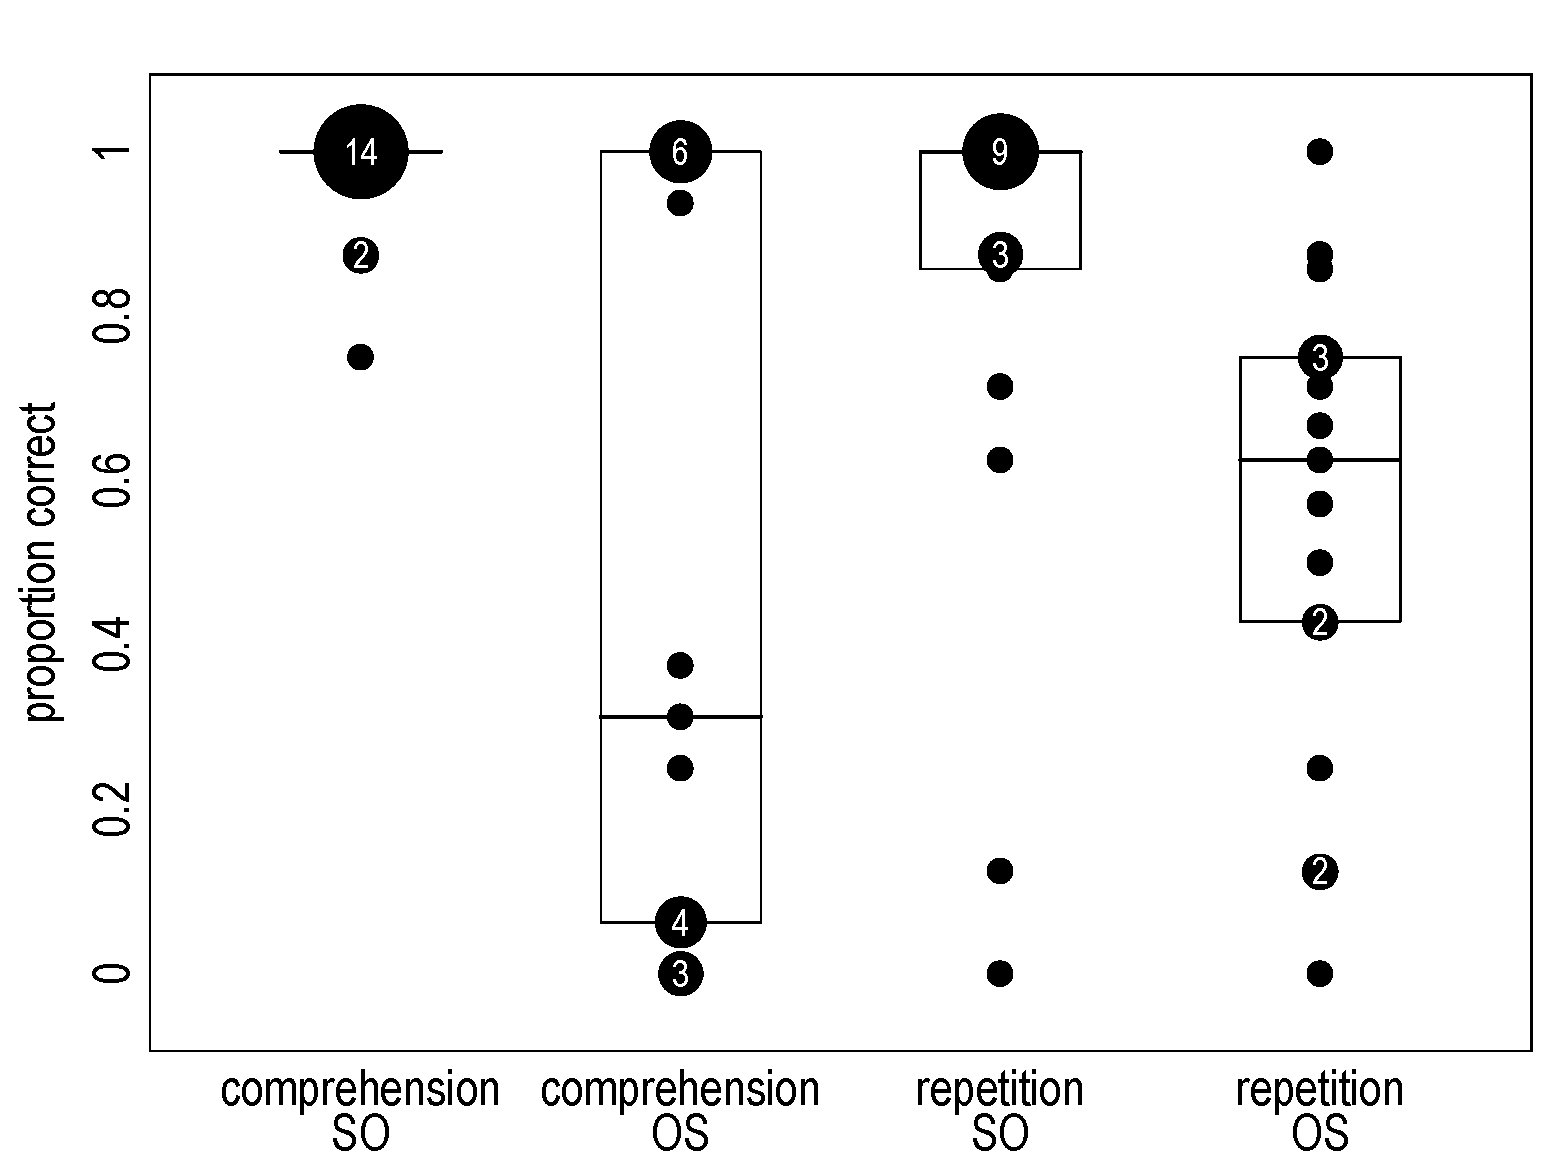
\includegraphics[width=\textwidth]{figures/06-1.pdf}
    \caption{Italian learners’ performance at T1, comprehension test and EIT}
    \label{fig:06:1}
\end{figure}

Moreover, differences in aggregated scores, even if proved to be statistically significant, do not necessarily have a linguistic interpretation. Finally, each graph only describes the performance of a single L1 group at either test time. In the case of a complex project such as VILLA, it would take ten such graphs to fully describe tendencies in the data-set.

To address this first limitation, \tabref{tab:06:1} presents the proportion of learners scoring statistically above chance in each test condition, based on the methodology described in \sectref{sec:04:2.4}.

\begin{table}
    \begin{tabularx}{\textwidth}{Xrrrrrrrrrrrrrrrr}
    \lsptoprule
    & \multicolumn{8}{c}{ OS} & \multicolumn{8}{c}{ SO}\\
    & \multicolumn{4}{c}{ T1} & \multicolumn{4}{c}{ T2} & \multicolumn{4}{c}{ T1} & \multicolumn{4}{c}{ T2}\\
    & \multicolumn{2}{c}{ Comp} & \multicolumn{2}{c}{ EI} & \multicolumn{2}{c}{ Comp} & \multicolumn{2}{c}{ EI} & \multicolumn{2}{c}{ Comp} & \multicolumn{2}{c}{ EI} & \multicolumn{2}{c}{ Comp} & \multicolumn{2}{c}{ EI}\\
    \midrule
    & + & {}- & + & {}- & + & {}- & + & {}- & + & {}- & + & {}- & + & {}- & + & {}-\\
    EN & 1 & 16 & 0 & 17 & 1 & 16 & 0 & 17 & 17 & 0 & 0 & 16 & 16 & 0 & 0 & 16\\
    FR & 4 & 13 & 0 & 17 & 9 & 8 & 2 & 15 & 16 & 1 & 1 & 16 & 14 & 3 & 5 & 12\\
    GE & 10 & 7 & 7 & 13 & 15 & 5 & 11 & 9 & 19 & 1 & 8 & 12 & 18 & 2 & 9 & 11\\
    IT & 7 & 10 & 6 & 11 & 11 & 6 & 8 & 9 & 17 & 0 & 13 & 4 & 17 & 0 & 14 & 3\\
    NL & 5 & 15 & 2 & 18 & 8 & 12 & 5 & 15 & 20 & 0 & 6 & 14 & 15 & 5 & 7 & 13\\
    \lspbottomrule
    \end{tabularx}
    \caption{Learners scoring above chance}
    \label{tab:06:1}
\end{table}

This time the data are arranged and interpreted in such a way that they have an immediate linguistic interpretation, that is, whether or not the learners can be thought to have applied a morphosyntactic strategy. Again, however, no information is provided as to the score of individual learners in various conditions.

\subsection{Scenarios}\label{sec:06:2.2}

In order to portray a comprehensive picture of learners’ morphosyntactic skills, “scenarios” (see \sectref{sec:03:2.4.3}\todo{No 2.4.3 in Chapter 4; only 2.4 and 2.4.1}) are introduced as a methodological tool. Scenarios represent a single, global score of the learners' processing skills in both comprehension and repetition. For each test, scores are coded as 'positive' or ‘negative’ based on the rationale described in section (SECTION)\todo{To be updated}. Four scenarios are possible (\tabref{tab:06:2}):
\begin{table}
    \begin{tabular}{|lc|cc|}
    \hline
    & & \multicolumn{2}{c|}{ comprehension}\\
    &  & $+$ & $-$\\
    \hline
     \multirow{2}{*}{repetition} & $+$ & \textbf{1} & \textbf{4}\\
                                & $-$ & \textbf{3} & \textbf{2}\\
    \hline
    \end{tabular}
    \caption{Scenarios, rationale}
    \label{tab:06:2}
\end{table}

In scenarios 1 and 2, both tests are performed above chance and at or below chance level, respectively. Scenarios 2 and 4, in contrast, point to a situation in which learners perform well in one test and poorly in the other one. It is thus possible to investigate whether the two skills are correlated in the learners' competence, the alternative hypothesis being that either might develop earlier in time.

The use of this tool is exemplified on the basis of the results obtained by all learners at T1 on OS targets. The area of \figref{fig:06:2} is divided into four squares, each corresponding to a scenario, indicated by a large number in red. Learners are identified by a coloured digraph according to their L1 (\tabref{tab:06:3}).

\begin{table}
    \begin{tabularx}{\textwidth}{XXXXXX}
    \lsptoprule
    L1 & English & French & German & Italian & Dutch\\
    Identifier & EN & FR & GE & IT & NL\\
    Colour & red & blue & black & green & orange\\
    \lspbottomrule
    \end{tabularx}
    \caption{\figref{fig:06:2}, identifiers}
    \label{tab:06:3}
\end{table}

Depending on whether or not the performance of the learner in question varies from T1 to T2 or not, the digraph is printed in lowercase or uppercase letters, respectively. Learners identified by capital letters will no longer be in the same position in the graph depicting the situation at T2 (\figref{fig:06:3}), while those identified by small letters remain in the same square at both T1 and T2. 

Crucially, participants are identified univocally by their position in the graph, at the intersection of their comprehension and repetition scores. The position of each learner in the square does not reflect actual scores in the two tests: rather, for the reasons previously discussed, the graph only indicates the participants’ performance in terms of scenarios. Their position within each square is simply meant to improve readability. 

\begin{figure}
    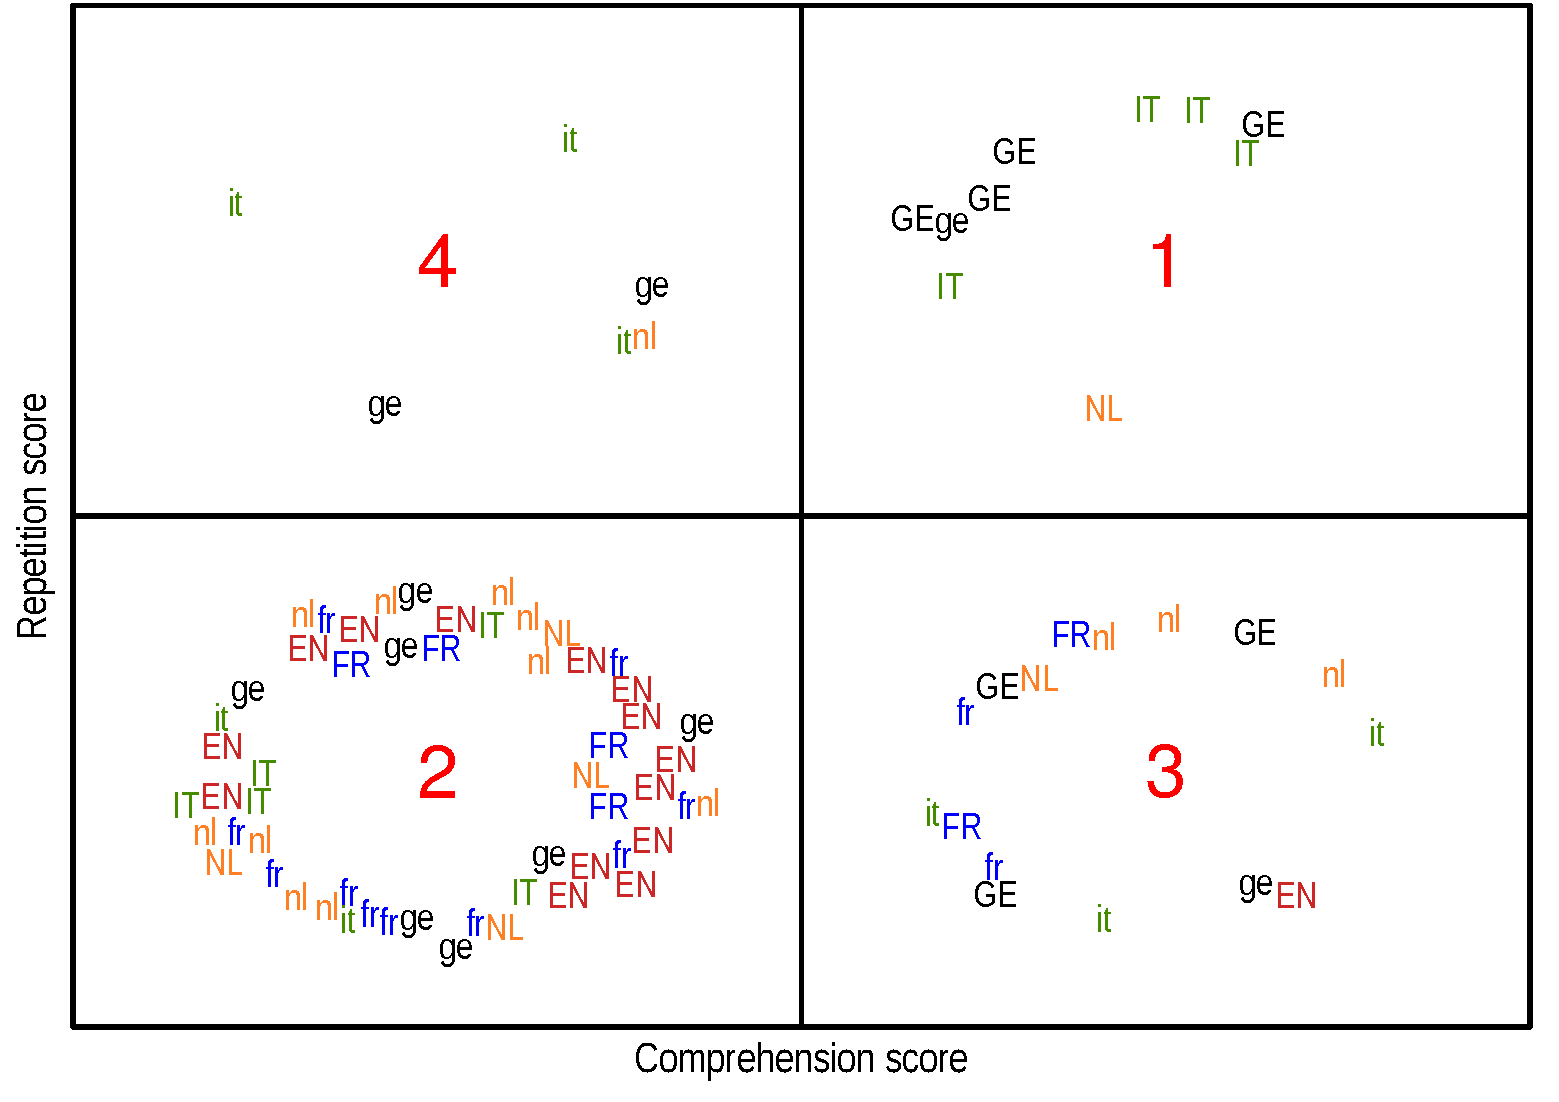
\includegraphics[width=\textwidth]{figures/06-2.pdf}
    \caption{Repetition and comprehension scores, OS targets, Time 1}
    \label{fig:06:2}
\end{figure}

An obvious cluster comprising more than a half of the dataset at T1 is located in scenario 2, indicating that neither test was performed with above chance accuracy. The second largest cluster corresponds to scenario 3, indicating above chance scores in comprehension, but not in repetition. Finally, a smaller group of learners can be found in scenario 1, indicating that already at T1 some learners managed to process OS targets morpho-syntactically in both comprehension and repetition. Coherently with the assumptions of the EI task, very few learners are found in scenario 4, which corresponds to above chance performance in repetition, but not in comprehension.

The picture presented so far is still incomplete, as it only depicts learner performance on OS targets. In order to provide a comprehensive picture of learners' processing, though, it would be desirable to have a synoptic representation of performance on SO targets as well. 

This may be exemplified by focussing on the learners located in scenario 2 in \figref{fig:06:2} (scoring at or below chance level for both comprehension and production). \figref{fig:06:3} depicts their performance on SO targets following the same rationale. 

\begin{figure}
    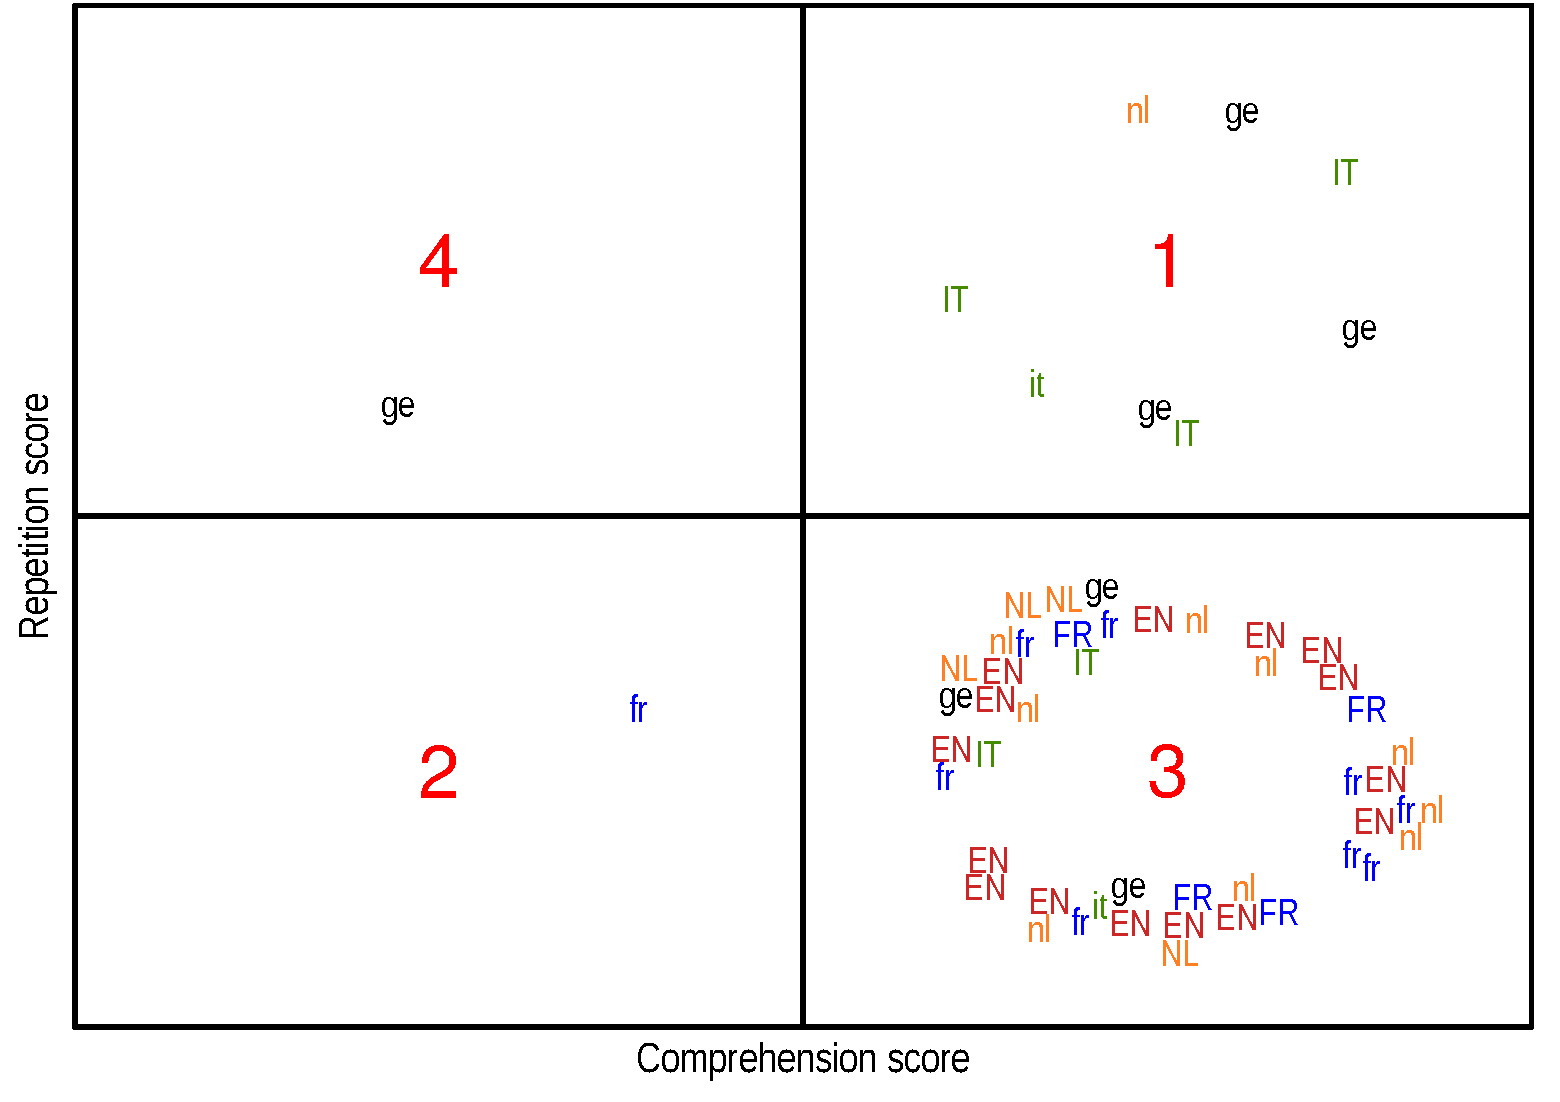
\includegraphics[width=\textwidth]{figures/06-3.pdf}
    \caption{Repetition and comprehension scores on SO targets for learners in sc. 2 on OS targets, Time 1}
    \label{fig:06:3}
\end{figure}

Again, an obvious cluster can be identified, this time in scenario 3. Such good performance on SO targets is hardly surprising, as target-like interpretation may be achieved based on either a positional or a morphosyntactic principle. The exiguity of data points in scenario 1, in contrast, witnesses to the greater difficulty of the EI task, although 8 learners do exhibit above chance accuracy. Finally, Scenarios 2 and 4 violate the assumptions of both test rationale and word order manipulation and are coherently empty.

The next step consists in merging the information presented in \figref{fig:06:2} and \figref{fig:06:3} into a single, comprehensive representation. This is achieved as shown in \figref{fig:06:4}.

\begin{figure}
    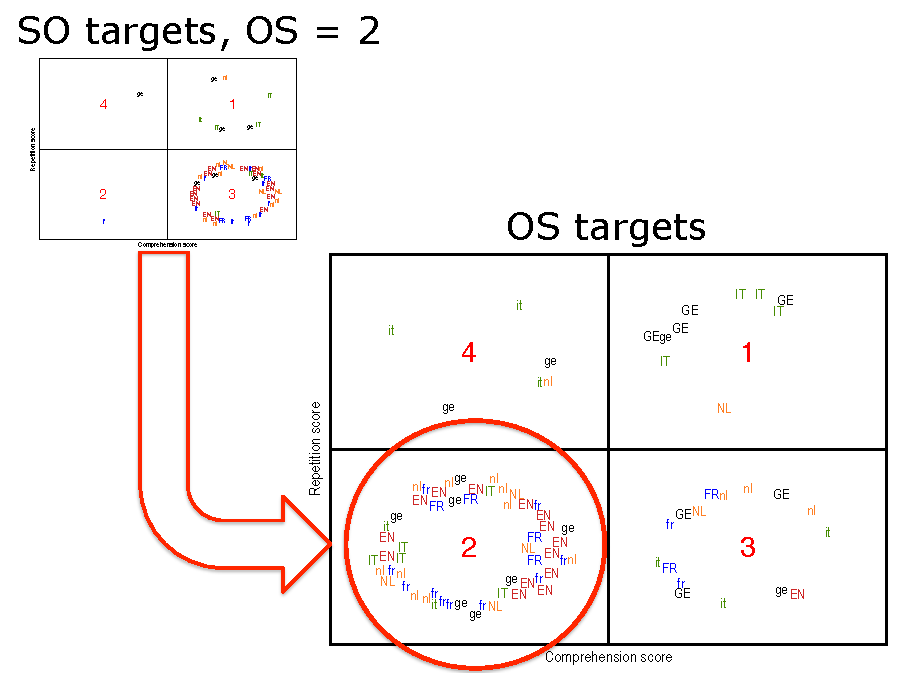
\includegraphics[width=\textwidth]{figures/06-4.pdf}
    \caption{Merging the information presented in \figref{fig:06:2} and \figref{fig:06:3}}
    \label{fig:06:4}
\end{figure}

The main squares of the graph representing the processing of OS targets are further divided into 4 minor squares, depicting the processing of SO targets by the learners comprised in the main square. Both representations rely on scenarios, arranged clockwise (4,1,3,2) for both targets, where 1 represents above-chance performance in both tests, 2 under-chance performance in both tests, and 3 and 4 depicting the situation of learners who perform above chance in one test and below in the other. To exemplify, scenario 2 on OS targets comprises 57 learners (circled in red). Based on their performance on SO targets, these learners may be grouped as follows: sc. 4: 1; sc. 1: 8; sc. 4: 1, sc. 3: 47. This distribution is graphically represented by the small square on the top left. But it would also be useful to show the performance of each learner on both SO and OS targets at the same time: to this purpose, the representation in the red circle, which only indicates sc. 2 performance on OS targets, is substituted with the square on the top left, which adds information as to the same learners’ performance on SO targets. The final result is shown in \figref{fig:06:5}.

\begin{figure}
    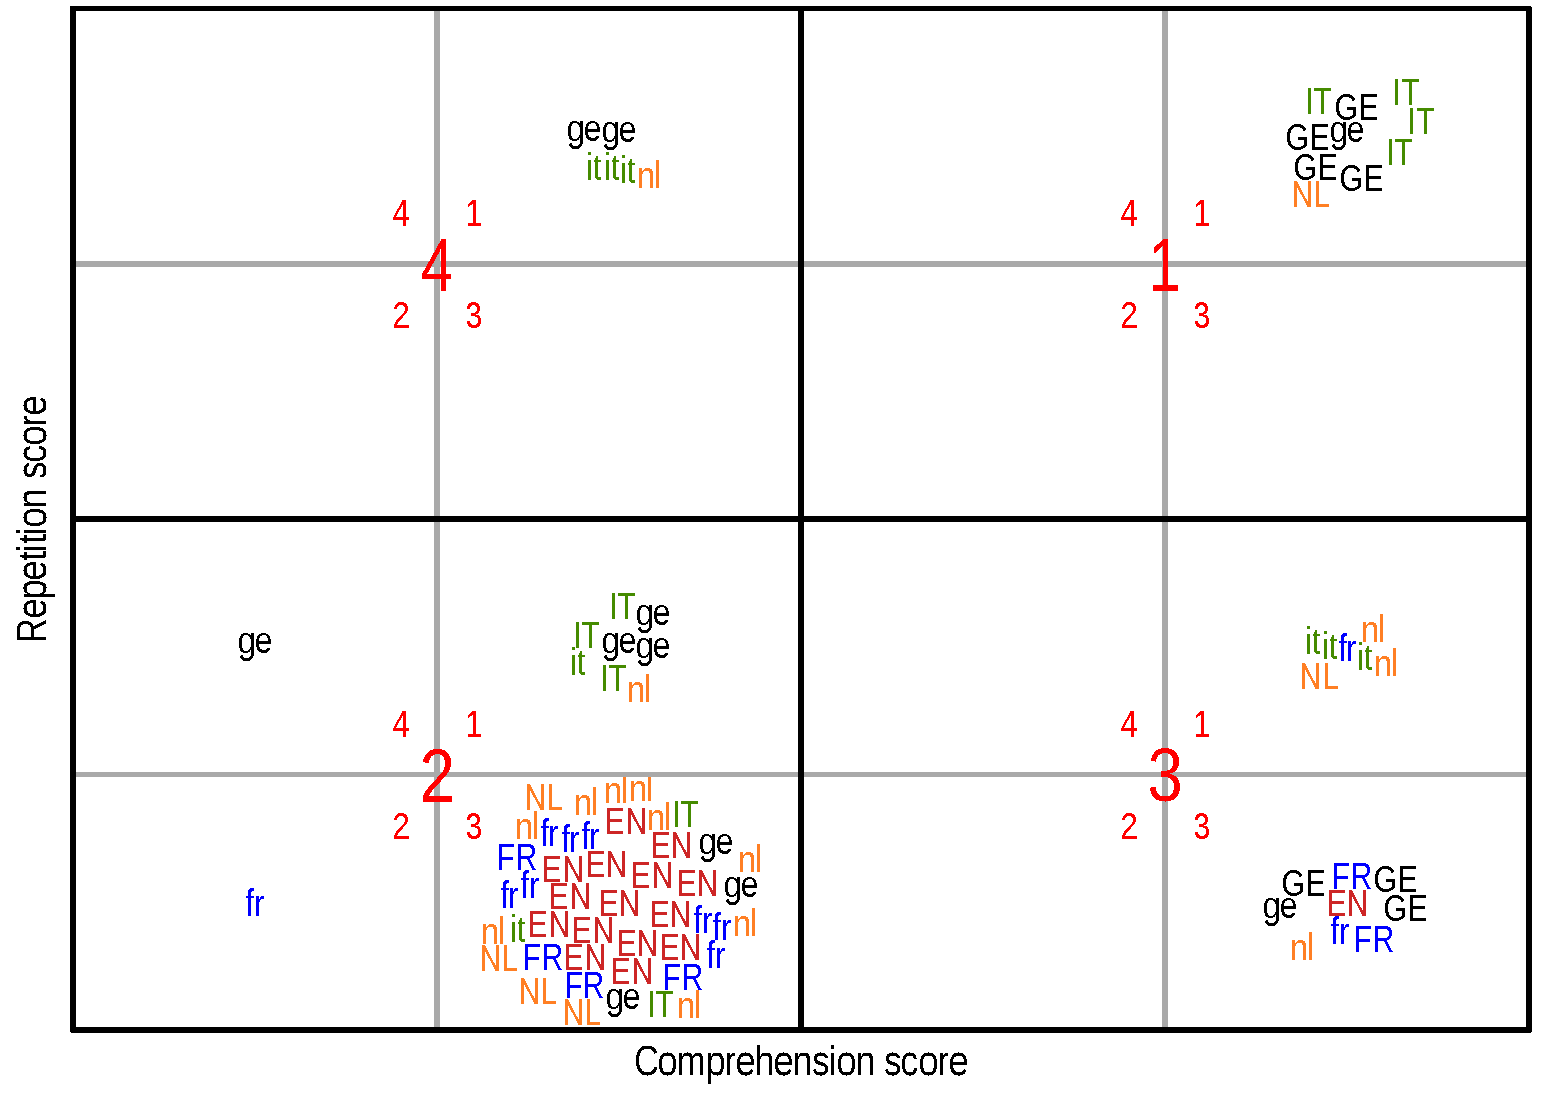
\includegraphics[width=\textwidth]{figures/06-5.pdf}
    \caption{Scenarios, T1}
    \label{fig:06:5}
\end{figure}

\section{An overall picture of learner morphosyntactic skills: results}\label{sec:06:3}

\figref{fig:06:5} is divided into 16 squares, which correspond to unique combinations of OS and SO processing scores. Each square is identified by two coordinates, corresponding to the OS scenario (large numbers) followed by the SO scenario (smaller numbers). To exemplify, scenario 2;3 corresponds to the largest cluster observed (second from left, bottom row). Again, some of the theoretically possible scenarios are linguistically unmotivated, and are accordingly empty. A rationale of linguistically motivated scenarios is provided below.

\begin{itemize}
    \item[1;1] Full morphosyntactic principle. Both tests are performed with above chance accuracy on both types of targets.
    \item [3;1] On SO targets, both tests are performed above chance; with OS targets, only the comprehension test is. The repetition of OS targets proves the hardest task.
    \item[2;1] Both tests are performed with above chance accuracy on SO targets; on OS targets, neither is. Independently of the test, OS targets are harder than SO ones.
    \item[2;3] Positional principle. only the comprehension test on SO targets is performed with above chance accuracy. 
\end{itemize}

The scenarios identified in \figref{fig:06:5} are represented analytically in \tabref{tab:06:4}. Each is broken down into its test and word order components. The last row computes the number of learners who perform above chance in each combination of test and word order. 

\begin{table}
    \fittable{
    \begin{tabular}{ccccrr}
    \lsptoprule
     OS repetition & SO repetition & OS comprehension & SO comprehension & scenario & n. \\
    \midrule
     + & + & + & + & 1;1 & 10\\
     -- & + & + & + & 3;1 & 7\\
     -- & -- & + & + & 2;1 & 8\\
     -- & -- & -- & + & 2;3 & 47\\
     + & -- & + & + & 4;1 & 5\\
     -- & + & -- & + & 3;3 & 9\\
     -- & -- & + & -- & 2;4 & 1\\
     -- & -- & -- & -- & 2;2 & 1\\
     \midrule
     15 & 26 & 31 & 86 &  & \\
    \lspbottomrule
    \end{tabular}
    }
    \caption{Implicational hierarchy at T1}
    \label{tab:06:4}
\end{table}

Following \citeauthor{AldaiWichmann2018} (\citeyear{AldaiWichmann2018}; see also \citealt{Nyqvist2018, Wichmann2015, Wichmann2016}; \citealt[210-212]{HatchLazaraton1991}), the matrix was submitted to a significance test of the degree of scalarity applying matrix randomization statistical testing (\citealt{JanssenEtAl2006}) based on Guttmann scaling. To this purpose, the R script made available by \citet{AldaiWichmann2018} as well as the \textit{vegan} R package \citep{OksanenEtAl2019} were used. A solid hierarchy emerges (GC 95,74, p < 0.01): 

OS repetition ${\supset}$ OS comprehension ${\supset}$ SO repetition ${\supset}$ SO comprehension. 

A few observations can be made. First, either task is harder on OS targets than on SO ones. Secondly, within a given constituent order, the EI task is harder than the comprehension test. Finally, all scenarios which are coherent with the hypotheses concerning constituent order and the EI task are indeed part of the hierarchy. There is an exception to this rule, however: scenario 3;3, comprising 9 learners, which is not part of the hierarchy and yet does not violate any assumption:

\begin{itemize}
    \item[3;3]  comprehension scores are above chance on both SO and OS targets, whereas repetition scores are at chance level. 
\end{itemize}

This scenario suggests that, independently of the target structure, repetition is harder for the learners than comprehension. Truly, it was not predicted that if learners can process OS targets in comprehension, they should be able to process SO targets in repetition, too. However, the vast majority appears to follow this pattern. Scenario 3;3 comprises 9 learners, whereas the closest scenario compatible with the hierarchy, namely 3;1 (success in comprehension on OS targets; success in both tests on SO targets), comprises 7 learners, so that the two situations seem equally possible. 

Another 5 learners are found in scenario 4;1, which contradicts the assumptions of the EI task: 

\begin{itemize}
    \item[4;1]  on SO targets, both tests are performed above chance; on OS targets repetition is above chance and comprehension is at chance level. 
\end{itemize}

The two remaining scenarios comprising a single learner each (2;4, 2;2) make little sense linguistically, and may be due to the participants’ lack of commitment or to random variation in their non-systematic responses. 

\subsection{Effects of additional exposure to the input}\label{sec:06:3.1}

The picture presented above describes the situation at T1 (9 hours). This section presents the results obtained after an additional 4h30 of instruction (T2). \figref{fig:06:6} presents the data in terms of scenarios.

\begin{figure}
    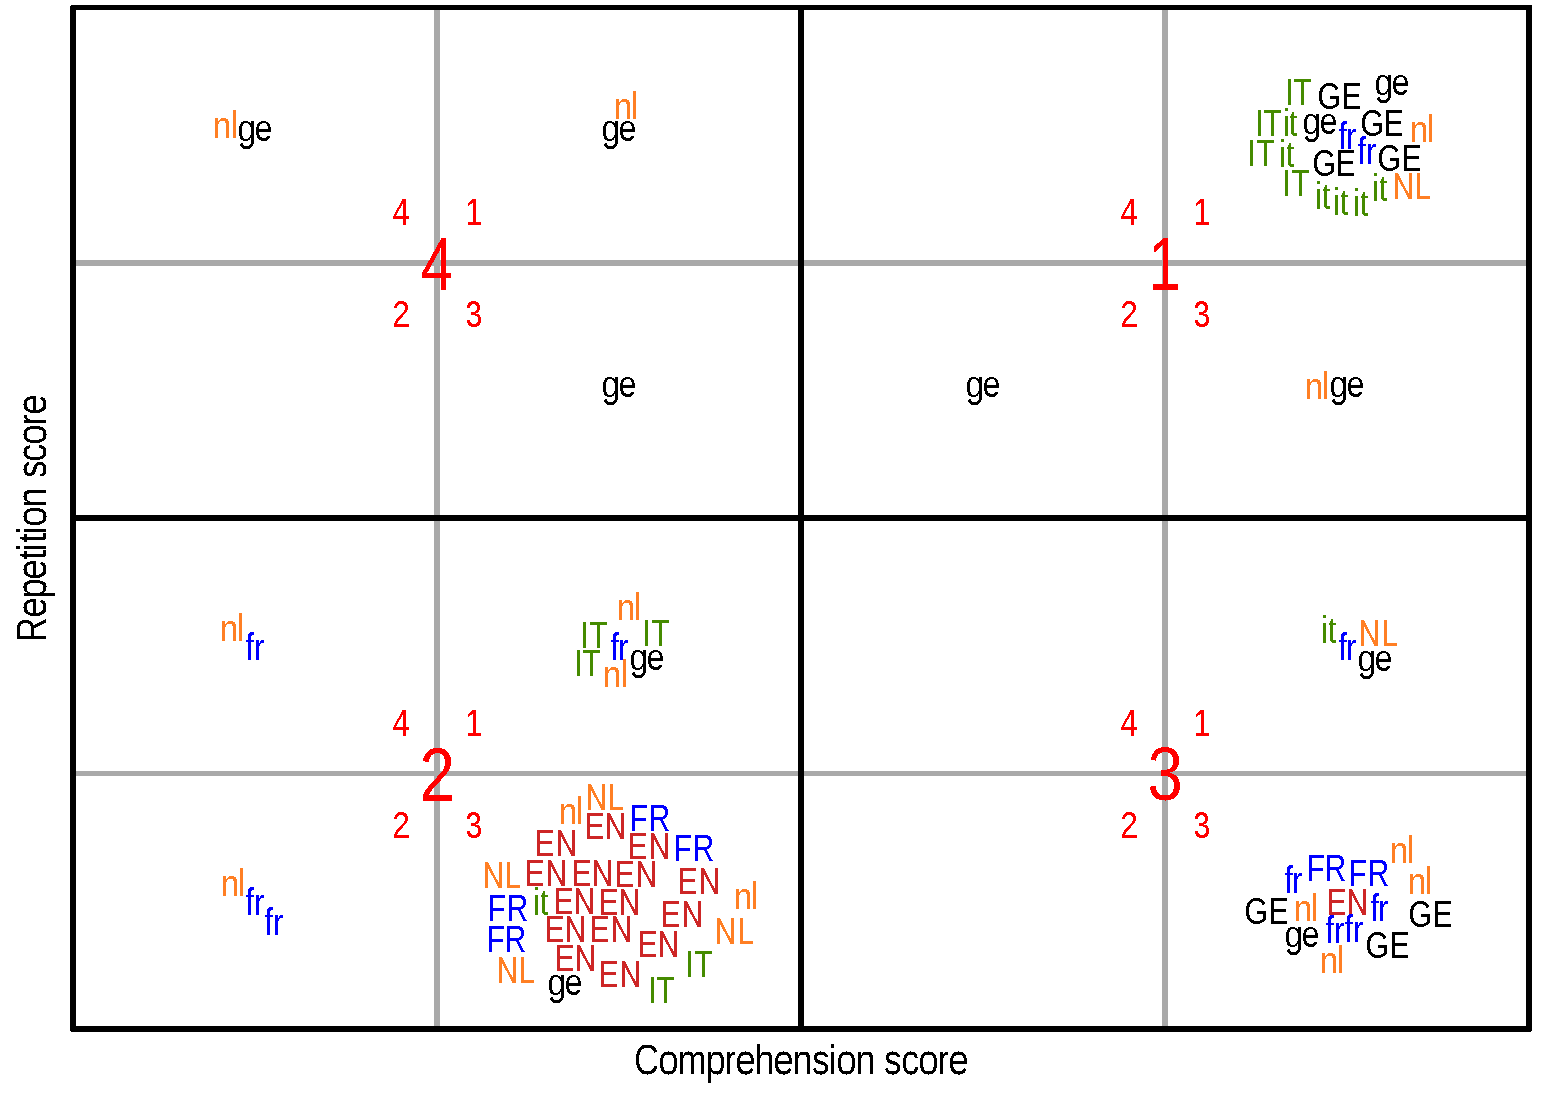
\includegraphics[width=\textwidth]{figures/06-6.pdf}
    \caption{Scenarios, T2}
    \label{fig:06:6}
\end{figure}

The main patterns observed at T1 seem to hold at T2 as well. The largest cluster still corresponds to scenario 2;3, although it now comprises fewer learners, whereas the cluster corresponding to a full morphosyntactic principle (1;1) nearly doubled. Finally, greater dispersion across scenarios is observed than at T1. The same tendencies are represented analytically in \tabref{tab:06:5}.\todo{Table 4 and 5 had both been named Table 4 and the rest had followed. Now fixed.}

\begin{table}
\fittable{
    \begin{tabular}{ccccrr}
    \lsptoprule
     OS repetition & SO repetition & OS comprehension & SO comprehension & scenario & n. \\
     \midrule
     + & + & + & + & 1;1 & 20\\
     -- & + & + & + & 3;1 & 4\\
     -- & + & -- & + & 2;1 & 7\\
     -- & -- & -- & + & 2;3 & 29\\
     + & -- & + & + & 1;3 & 2\\
     + & -- & + & -- & 1;2 & 1\\
     + & + & -- & + & 4;1 & 2\\
     + & -- & -- & + & 4;3 & 1\\
     + & + & -- & -- & 4;4 & 2\\
     -- & -- & + & + & 3;3 & 15\\
     -- & + & -- & -- & 2;4 & 2\\
     -- & -- & -- & -- & 2;2 & 3\\
     28 & 37 & 42 & 80 &  & 88\\
    \lspbottomrule
    \end{tabular}
    }
    \caption{Implicational hierarchy at T2}
    \label{tab:06:5}
\end{table}

Scalability analysis (GC = 92.9, p < 0,01) indicates a slightly different hierarchy than observed at T1:

OS repetition ${\supset}$ SO repetition ${\supset}$ OS comprehension ${\supset}$ SO comprehension. 

The effect of task at T2 thus appears to be slightly more relevant than that of word order, whereas the opposite was true at T1. Nevertheless, it should be pointed out that the difference between the second and the third step of the scale is minimal (5 learners at both test times).

Moving further, it is worthwhile to investigate whether any regularities may be detected in the evolution of learner processing strategies over time. Evolution patterns will be represented as a combination of the scenarios in which a learner is found at T1 and T2. 

The first column of \tabref{tab:06:6} ("pattern") lists all observed combinations of scenarios evolving from T1 to T2. This set comprises 30 items, a small fraction of the full set of possible combinations, amounting to 256 patterns, which shows that evolutionary patterns are not random

The second column shows the proportion of learners adopting each pattern. In the following columns, proportions are computed on the basis of each L1.

\begin{table}
\fittable{
    \begin{tabular}{lrrrrrr}
    \lsptoprule
    
    pattern & tot (n=88) & EN (n=16) & FR (n=17) & GE (n=18) & IT (n=17) & NL (n=20)\\
    \midrule
    2\_3 2\_3 & 28\% & 94\% & 24\% & 0\% & 12\% & 20\%\\
    1\_1 1\_1 & 10\% & 0\% & 0\% & 22\% & 24\% & 5\%\\
    2\_3 3\_3 & 8\% & 0\% & 24\% & 6\% & 0\% & 10\%\\
    3\_3 3\_3 & 7\% & 6\% & 12\% & 17\% & 0\% & 0\%\\
    3\_1 1\_1 & 5\% & 0\% & 6\% & 0\% & 18\% & 0\%\\
    2\_1 2\_1 & 3\% & 0\% & 0\% & 0\% & 18\% & 0\%\\
    2\_3 1\_1 & 3\% & 0\% & 0\% & 6\% & 6\% & 5\%\\
    2\_3 2\_1 & 3\% & 0\% & 6\% & 0\% & 0\% & 10\%\\
    2\_3 2\_2 & 3\% & 0\% & 12\% & 0\% & 0\% & 5\%\\
    2\_1 2\_3 & 2\% & 0\% & 0\% & 0\% & 6\% & 5\%\\
    2\_3 4\_4 & 2\% & 0\% & 0\% & 6\% & 0\% & 5\%\\
    3\_1 3\_3 & 2\% & 0\% & 0\% & 0\% & 0\% & 10\%\\
    4\_1 1\_1 & 2\% & 0\% & 0\% & 0\% & 12\% & 0\%\\
    1\_1 1\_2 & 1\% & 0\% & 0\% & 6\% & 0\% & 0\%\\
    2\_1 1\_1 & 1\% & 0\% & 0\% & 6\% & 0\% & 0\%\\
    2\_1 1\_3 & 1\% & 0\% & 0\% & 6\% & 0\% & 0\%\\
    2\_1 4\_1 & 1\% & 0\% & 0\% & 6\% & 0\% & 0\%\\
    2\_2 2\_4 & 1\% & 0\% & 6\% & 0\% & 0\% & 0\%\\
    2\_3 2\_4 & 1\% & 0\% & 0\% & 0\% & 0\% & 5\%\\
    2\_3 3\_1 & 1\% & 0\% & 6\% & 0\% & 0\% & 0\%\\
    2\_3 4\_1 & 1\% & 0\% & 0\% & 0\% & 0\% & 5\%\\
    2\_4 2\_3 & 1\% & 0\% & 0\% & 6\% & 0\% & 0\%\\
    3\_1 3\_1 & 1\% & 0\% & 0\% & 0\% & 0\% & 5\%\\
    3\_3 1\_1 & 1\% & 0\% & 6\% & 0\% & 0\% & 0\%\\
    3\_3 1\_3 & 1\% & 0\% & 0\% & 0\% & 0\% & 5\%\\
    3\_3 3\_1 & 1\% & 0\% & 0\% & 6\% & 0\% & 0\%\\
    4\_1 2\_1 & 1\% & 0\% & 0\% & 6\% & 0\% & 0\%\\
    4\_1 2\_3 & 1\% & 0\% & 0\% & 0\% & 0\% & 5\%\\
    4\_1 3\_1 & 1\% & 0\% & 0\% & 0\% & 6\% & 0\%\\
    4\_1 4\_3 & 1\% & 0\% & 0\% & 6\% & 0\% & 0\%\\
    \lspbottomrule
    \end{tabular}
    }
    \caption{Patterns of morphosyntactic processing over time}
    \label{tab:06:6}
\end{table}

The first striking observation regards the lack of clear cross-linguistic patterns in the data. Second, among the five most common patterns, three - comprising 28\%, 10\% and 7\% of the data respectively - indicate no change between T1 and T2. Next, the English L1 group is the most homogeneous - all learners but one are found in scenario 2;3, corresponding to a clear positional principle, and all learners show now change at all from T1 to T2. All other language groups exhibit more dispersion, with most clusters comprising just a single learner, and some representing a few learners. 

\section{Inferential statistics}\label{sec:06:4}

To statistically verify the tendencies identified so far, a generalised linear mixed model with binomial error structure and logit link function (Likelihood Type 3-test) was fitted to the data. The dependent variable is given by a matrix reporting each learner’s successes and failures for a given combination of predictors. Control predictors include task type (binary factor, reference level=EIT), word order (binary factor, reference level=OS), L1 (factor, EN, FR, GE, IT, NL, reference level=ENG) and test time (binary factor, reference level=T1). The interactions which proved significant in the previous analyses (i.e. L1:word order and time:word order, see sections \ref{sec:04:2.3} and \ref{sec:05:2.1}) were also added. The model is designed to test the two-way interactions concerning the predictor “task”, i.e. task:time, task:word order, task:L1, whose underlying hypothesis is that the effect of task type varies depending on target sentence word order, test time and learner L1, respectively. 

Random effects include random intercepts for participants and target items as well as correlated random slopes for time, test time and test type. 

Convergence issues unfortunately made it impossible to include a more complex structure. The summary of the model is presented in \tabref{tab:06:7}.

\begin{table}
    \begin{tabularx}{\textwidth}{Xrrr}
    \lsptoprule
    \textbf{~} & \multicolumn{3}{c}{ \textbf{mat}}\\
    \textit{Predictors} & \textit{Odds} \textit{Ratios} & \textit{CI} & \textit{p}\\
    \midrule
    (Intercept) & 0.06 & 0.02~–~0.17 & \textbf{<0.001}\\
    time & 3.13 & 2.27~–~4.33 & \textbf{<0.001}\\
    L1 [FR] & 3.27 & 0.77~–~13.89 & 0.108\\
    L1 [GE] & 15.64 & 3.86~–~63.46 & \textbf{<0.001}\\
    L1 [IT] & 8.37 & 1.89~–~37.05 & \textbf{0.005}\\
    L1 [NL] & 2.52 & 0.63~–~10.20 & 0.193\\
    WO2 [SO] & 315.01 & 135.99~–~729.67 & \textbf{<0.001}\\
    test [EIT] & 0.06 & 0.02~–~0.21 & \textbf{<0.001}\\
    WO2 [SO] * test [EIT] & 0.07 & 0.04~–~0.10 & \textbf{<0.001}\\
    L1 [FR] * test [EIT] & 4.35 & 0.93~–~20.43 & 0.062\\
    L1 [GE] * test [EIT] & 18.74 & 4.12~–~85.13 & \textbf{<0.001}\\
    L1 [IT] * test [EIT] & 16.60 & 3.40~–~81.05 & \textbf{0.001}\\
    L1 [NL] * test [EIT] & 12.92 & 2.91~–~57.40 & \textbf{0.001}\\
    time * test [EIT] & 0.77 & 0.54~–~1.08 & 0.126\\
    time * WO2 [SO] & 0.46 & 0.32~–~0.64 & \textbf{<0.001}\\
    L1 [FR] * WO2 [SO] & 0.34 & 0.15~–~0.80 & \textbf{0.012}\\
    L1 [GE] * WO2 [SO] & 0.06 & 0.03~–~0.14 & \textbf{<0.001}\\
    L1 [IT] * WO2 [SO] & 1.01 & 0.40~–~2.55 & 0.979\\
    L1 [NL] * WO2 [SO] & 0.44 & 0.20~–~0.97 & \textbf{0.042}\\
    \multicolumn{4}{c}{\textbf{Random} \textbf{Effects}}\\
    σ\textsuperscript{2} & \multicolumn{3}{c}{3.29}\\
    τ\textsubscript{00}~\textsubscript{participant} & \multicolumn{3}{c}{3.30}\\
    τ\textsubscript{00}~\textsubscript{participant.1} & \multicolumn{3}{c}{1.00}\\
    τ\textsubscript{00}~\textsubscript{participant.2} & \multicolumn{3}{c}{2.19}\\
    τ\textsubscript{11}~\textsubscript{participant.testEIT} & \multicolumn{3}{c}{4.03}\\
    τ\textsubscript{11}~\textsubscript{participant.1.WO2SO} & \multicolumn{3}{c}{0.52}\\
    τ\textsubscript{11}~\textsubscript{participant.2.time} & \multicolumn{3}{c}{1.30}\\
    ρ\textsubscript{01}~\textsubscript{participant} & \multicolumn{3}{c}{{}-0.82}\\
    ρ\textsubscript{01}~\textsubscript{participant.1} & \multicolumn{3}{c}{{}-1.00}\\
    ρ\textsubscript{01}~\textsubscript{participant.2} & \multicolumn{3}{c}{{}-1.00}\\
    ICC & \multicolumn{3}{c}{0.41}\\
    N~\textsubscript{participant} & \multicolumn{3}{c}{91}\\
    Observations & \multicolumn{3}{c}{720}\\
    Marginal R\textsuperscript{2}~/ Conditional R\textsuperscript{2} & \multicolumn{3}{c}{0.494 / 0.704}\\
    \lspbottomrule
    \end{tabularx}
    \caption{Model output}
    \label{tab:06:7}
\end{table}

The interactions involving the predictor “test” were tested by comparing the full model described above to three reduced models, each lacking the single interaction of interest (\tabref{tab:06:8}).

\begin{table}
    \begin{tabularx}{\textwidth}{XXXr}
    \lsptoprule
    predictor & Chisq & Df & Pr(>Chisq)\\
    \midrule
    task : word order & 191.892 & 1 & < 0.01\\
    task : L1 & 17.557 & 4 & < 0.01\\
    task : time & 2.339 & 1 & > 0.05\\
    \lspbottomrule
    \end{tabularx}
    \caption{Single-term deletion}
    \label{tab:06:8}
\end{table}

Pairwise comparisons show that the predictors interact in a complex way, producing numerous statistically significant contrasts. Performance in the two tasks was usually statistically significant, which confirms the initial hypothesis that the EIT is indeed more demanding than the comprehension task. The only contrasts which proved \textit{not} significant involved the OS word order and the German, Italian and Dutch L1 groups at both test times.

\subsection{Repetition in the absence of comprehension}\label{sec:06:4.1}

The rationale of the analysis presented so far is that learner comprehension and repetition scores combined should provide a comprehensive picture of the principles of utterance organisation observable in the learner variety. The validity of this approach relies on the assumptions of the EI task, namely that target repetition is impossible without its comprehension. Phonological memory should not play any significant role in this test. 

Nevertheless, a few learners appear to violate this assumption. For each relevant combination of test time and word order, \tabref{tab:06:9} provides comprehension and repetition scores of learners who at least at one test time appeared in scenario 4, along with the probability of observing such a distribution in the absence of a rational morpho-syntactic principle. Information as to the learners' performance in terms of scenarios at T1 and T2 is also provided in the last two columns. The table shows that repetition and comprehension scores are consistently very high or very low, which excludes the possibility that the subject were assigned to scenario 4 only because they slightly exceeded score thresholds. 

\begin{table}
\fittable{
    \begin{tabular}{lllllllllll}
    \lsptoprule
    & time & WO & subj. & L1 & rep. score & rep. p & comp. score & comp. p & sc. T1 & sc. T2\\
    \midrule
    a. & 1 & OS & 2108 & NL & 0.88 & < 0.01 & 0.00 & 1.00 & 4\_1 & 2\_3\\
    b. & 1 & OS & 4105 & GE & 0.80 & 0.03 & 0.44 & 0.60 & 4\_1 & 4\_3\\
    c. & 1 & OS & 4108 & GE & 0.83 & 0.02 & 0.31 & 0.89 & 4\_1 & 2\_1\\
    d. & 1 & OS & 5104 & IT & 0.71 & 0.06 & 0.38 & 0.77 & 4\_1 & 1\_1\\
    e. & 1 & OS & 5106 & IT & 0.75 & 0.04 & 0.00 & 1.00 & 4\_1 & 3\_1\\
    f. & 1 & OS & 5109 & IT & 0.86 & 0.01 & 0.00 & 1.00 & 4\_1 & 1\_1\\
    g. & 2 & OS & 2118 & NL & 0.88 & < 0.01 & 0.00 & 1.00 & 2\_3 & 4\_1\\
    h. & 2 & OS & 4105 & GE & 1.00 & < 0.01 & 0.31 & 0.89 & 4\_1 & 4\_3\\
    i. & 2 & OS & 4110 & GE & 1.00 & < 0.01 & 0.31 & 0.89 & 2\_1 & 4\_1\\
    l. & 1 & SO & 4112 & GE & 1.00 & < 0.01 & 0.50 & 0.36 & 2\_4 & 2\_3\\
    m. & 2 & SO & 1119 & FR & 0.75 & 0.04 & 0.12 & 0.96 & 2\_2 & 2\_4\\
    n. & 2 & SO & 2115 & NL & 0.88 & < 0.01 & 0.14 & 0.94 & 2\_3 & 2\_4\\
    \lspbottomrule
    \end{tabular}
    }
    \caption{Learners in scenario 4}
    \label{tab:06:9}
\end{table}

Participants in scenarios 2;4 and 4;4 exhibit higher scores in repetition than comprehension. This behaviour is hardly explicable in that they fail to score above chance in the comprehension of SO targets, which can be indifferently processed based on word order or inflectional morphology. A single participant is located in scenario 4;3, which surprisingly indicates above chance repetition of OS, but not SO targets, and just the opposite situation in the comprehension test. Such behaviour seems rather erratic and does not lend itself to a specific explanation. It must be mentioned, nevertheless, that results may slightly inflated because of repeated statistical testing. 

The facts reported above should induce a little caution as to the assumptions of the EI task. This section therefore aims to verify whether or not it is really possible to perform the EI task in the absence of comprehension. To this end, the VILLA EI task was administered to new groups of Italian, French and German participants selected on the basis of the VILLA guidelines (see \sectref{sec:06:2.3}\todo{No such section!})\footnote{Italian participants were recruited by the authour with the help of prof. Bernini and tested at the University of Bergamo; French and German participants were recruited and tested by Marzena Wątorek at the CNRS SFL, Paris, and by Christine Dimroth and Johanna Hinz at Münster University, respectively. Sincere thank to all of them for their helpful effort.}. These new test-takers were not exposed to any Polish input, so that it was impossible for them to process target sentences for meaning: the only skills they brought to the task was their phonological memory. Their performance therefore should be comparable to that of a VILLA subject who did not process targets for meaning, but only repeated them as a string of sounds. Will these participants with no comprehension skills be able to repeat ACC case endings? If that were the case, we should conclude that the VILLA EI task does not fulfil the assumptions of this kind of task.

A few examples of repetitions of the target sentence in \REF{ex:06:4a} are presented in (\ref{ex:06:4b}-d).

\ea%4
    \label{ex:06:4}
    \ea\label{ex:06:4a}
    \gll    /ʥevˈʧɨnk-e  ˈʨɔngnje  portuˈgalk-a/ \\
            little.girl-\textsc{acc}   pulls     Portuguese.woman-\textsc{nom}\\
    \ex\label{ex:06:4b}
    [ˈʧefnie ne'tswo na portuˈgala] \hfill (German group, subject 2)
    \ex\label{ex:06:4c}
    [dʒiˈkinʧi ˈkɔnʧe portuˈgarʧe] \hfill (French group, subject 1)
    \ex\label{ex:06:4d}
    [tsipˈtirne ʧo portuˈgal kta] \hfill (Italian team, subject 3)
    \z
\z

The two non-transparent words /ʥevʧɨnke/ and /ʨɔngnje/ are hardly recognisable, whereas the transparent word in final position sounds decidedly closer to the target, although accurate repetitions only concern that part of the word which is recognisable in both the target language and the subject's L1, namely the stem /portugal/. Suffixes and inflectional endings are mostly omitted or substituted with random linguistic material. At the same time, in some cases the segments corresponding to case endings are correctly repeated, in spite of being attached to a more or less random sequence of sounds, as [e] in [tsiptirne] \REF{ex:06:4d}. Since processing for meaning is to be excluded, one has to admit that the repetition of those segments can only be due to phonological memory. This too, however, is by no means a rule: working memory also seems prone to errors and inaccuracies, as witnessed by [e] in [portugarʧe] in \REF{ex:06:4c} for target [a] in /portuˈgalka/.

Nevertheless, comparing the output of the VILLA learners to that of first-exposure participants is not necessarily a legitimate operation. The examples in (\ref{ex:06:5b}-m\todo{n updated as m. There was no item j in the manually created list.}) report the repetition of the target sentence in \REF{ex:06:5a} as performed by learners who perform above chance in repetition, but not comprehension. Leaving inflectional endings aside for the moment, the output produced by these learners is quite different from that of the informants in \REF{ex:06:4}, as lexical items are clearly recognisable and produced with considerable accuracy. The overall picture will be discussed and interpreted in the following \chapref{sec:7} on semi-spontaneous production.

\ea%5
    \label{ex:06:5}
    \ea\label{ex:06:5a}
    \gll    /ʥevˈʧɨnk-e   ˈʨɔngnje   portuˈgalk-a/\\
            little.girl-\textsc{acc}   pulls     Portuguese.woman-\textsc{nom}\\
    \ex\label{ex:06:5b}
    [dʒewˈʧɨnke ˈʧɔngnie portuˈgalka]
    \ex\label{ex:06:5c}
    [dʒewˈʧenkə portuˈgalska]
    \ex\label{ex:06:5d}
    [dʒewˈʧɨnknɛ ˈportu ˈporta ˈbazu port portuˈgalka]
    \ex\label{ex:06:5e}
    [dʒjefˈʧɨnka dʒ ˈʧɔɲɲe portuˈgalka]
    \ex\label{ex:06:5f}
    [dʒjefˈʧɨnka kn eh ˈʧɔɲe portuˈgalkon]
    \ex\label{ex:06:5g}
    [portuˈgalka]
    \ex\label{ex:06:5h}
    [dʒewˈʧinke ˈʧɔngnie portuˈgalka]
    \ex\label{ex:06:5i}
    [dʒewˈʧɨnə ˈʧorgo portuˈgalka]
    \ex\label{ex:06:5j}
    [dsziewˈʧɨnkɛ ˈʧgnie portuˈgalka]
    \ex\label{ex:06:5k}
    BLANK
    \ex\label{ex:06:5l}
    [portuˈgalka ˈʧɔɲe dʒefˈkinkje]
    \ex\label{ex:06:5m}
    [portuˈgalke ˈʧɔngnie dʒewˈʧɨnke]
    \z
\z

\section{Conclusion}\label{sec:06:5}

Clear tendencies emerge from the analysis of morphosyntactic skills in the structured tests, pointing to the relatively greater difficulty of the EI task and of OS targets. Even though the majority of learners consistently apply a positional principle of utterance organisation, it is an impressive result that at least a fraction of them seems to be able to apply a morphosyntactic principle after only 9 hours. Their number increases with additional, albeit limited input exposure, suggesting that even complex target structures may be acquired spontaneously with no explicit instruction and within only hours from the first contact with the target language.
